\chapter{Analyses avancées sur données réelles (v1+)}
\label{chap:advanced_real}
Au-delà du tableau de bord descriptif, une suite analytique dédiée applique des
méthodes modernes de \emph{machine learning} et de \emph{data mining} sur les
données réelles, enrichies de covariables. L'ensemble est reproductible via
\texttt{python scripts/run\_advanced.py}.

\section{Accord entre sources et fuite de données}
Les statistiques de suicide de l'OMS (2021) et le taux d'automutilation de l'IHME
GBD mesurent des phénomènes quasi identiques : leur corrélation est forte
(Pearson $r \approx 0{,}84$). Utiliser l'automutilation comme variable
explicative du suicide reviendrait donc à une \textbf{fuite de données} (\emph{data
leakage}). En la retirant des prédicteurs, la performance en validation croisée
chute de $R^2 \approx 0{,}75$ à $R^2 \approx 0{,}19$ : le premier chiffre était un
artefact. Cette correction est assumée et documentée plutôt que masquée.
\begin{figure}[ht]
    \centering
    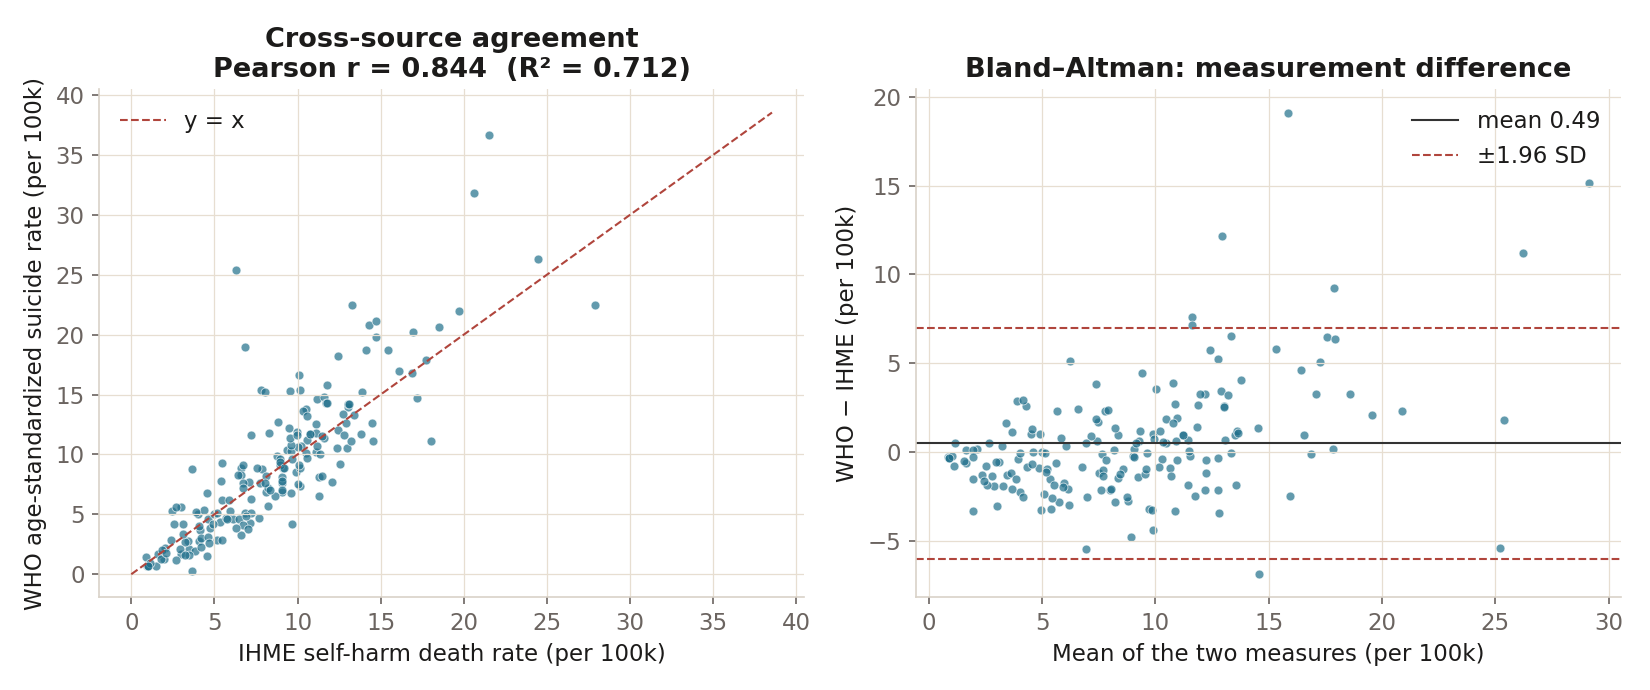
\includegraphics[width=\textwidth]{figures/fig_v1_source_agreement.png}
    \caption{Accord entre le suicide (OMS) et l'automutilation (IHME) : deux mesures presque redondantes.}
    \label{fig:v1_source_agreement}
\end{figure}

\section{Enrichissement par covariables}
Des covariables socio-économiques issues de la Banque mondiale (espérance de vie,
consommation d'alcool, etc.) sont ajoutées à la table pays. Après suppression de la
fuite, ces covariables deviennent les principaux facteurs explicatifs du modèle,
ce qui est cohérent avec la littérature de santé publique.

\section{Gradient boosting réglé et validation croisée imbriquée}
Un modèle LightGBM est optimisé par \textbf{Optuna} à l'intérieur d'une
\textbf{validation croisée imbriquée}, afin d'éviter toute fuite de réglage. Les
prédictions sont accompagnées :
\begin{itemize}
    \item d'attributions \textbf{SHAP} pour l'interprétabilité ;
    \item d'\textbf{intervalles conformes} (split-conformal), dont la couverture
    empirique ($\approx 96\%$) respecte la cible de 90\%.
\end{itemize}
Sur seulement 183 pays, un modèle linéaire régularisé reste compétitif : c'est un
constat honnête sur les limites d'un échantillon réduit.
\begin{figure}[ht]
    \centering
    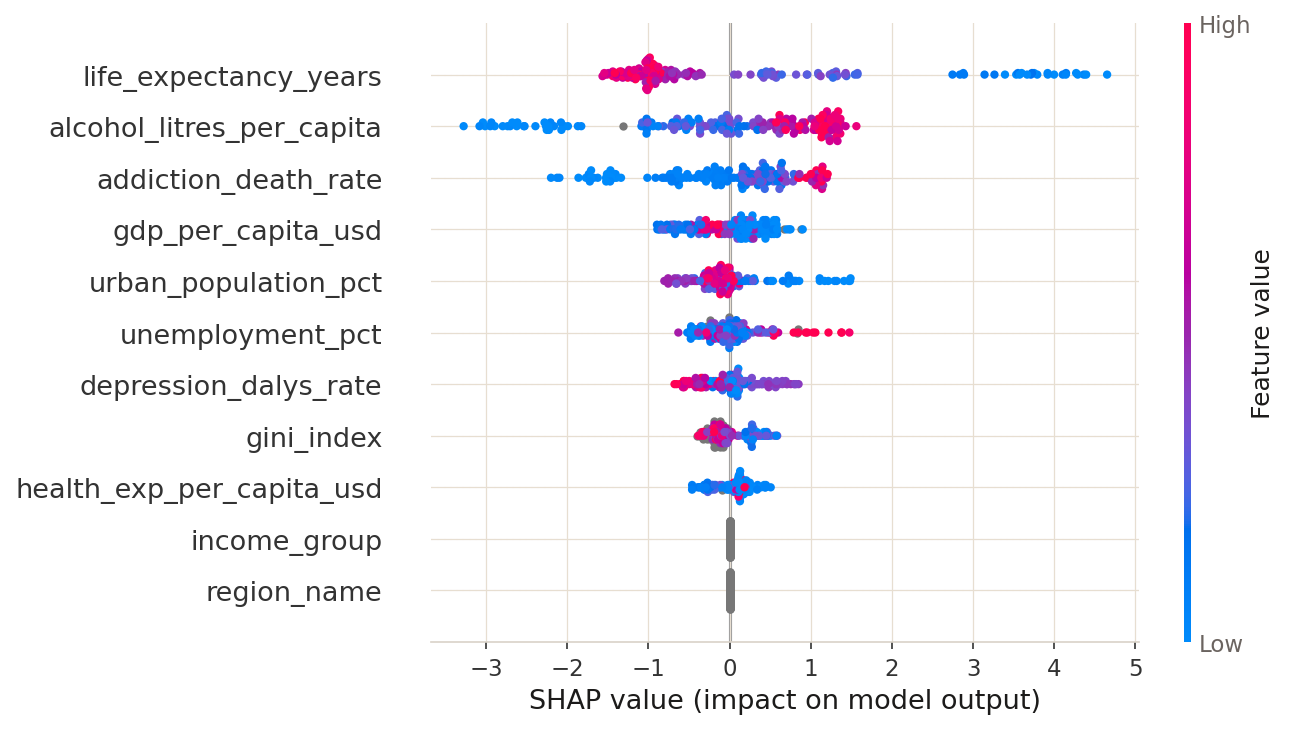
\includegraphics[width=\textwidth]{figures/fig_v1_shap_summary.png}
    \caption{Attributions SHAP : l'espérance de vie et l'alcool ressortent comme principaux facteurs.}
    \label{fig:v1_shap_summary}
\end{figure}

\section{Modèle hiérarchique à effets mixtes}
Un modèle à effets mixtes applique un \emph{partial pooling} des pays au sein des
régions OMS. Le coefficient de corrélation intra-classe ($\mathrm{ICC} \approx 0{,}22$)
quantifie proprement le regroupement géographique : c'est le traitement
statistiquement correct de données emboîtées.

\section{Réduction de dimension et réseau de similarité}
Une projection \textbf{UMAP} positionne les pays selon leur profil de santé
mentale, et un \textbf{réseau de similarité} (k plus proches voisins) révèle des
communautés de pays (modularité $\approx 0{,}72$) ainsi que des pays « ponts ».
\begin{figure}[ht]
    \centering
    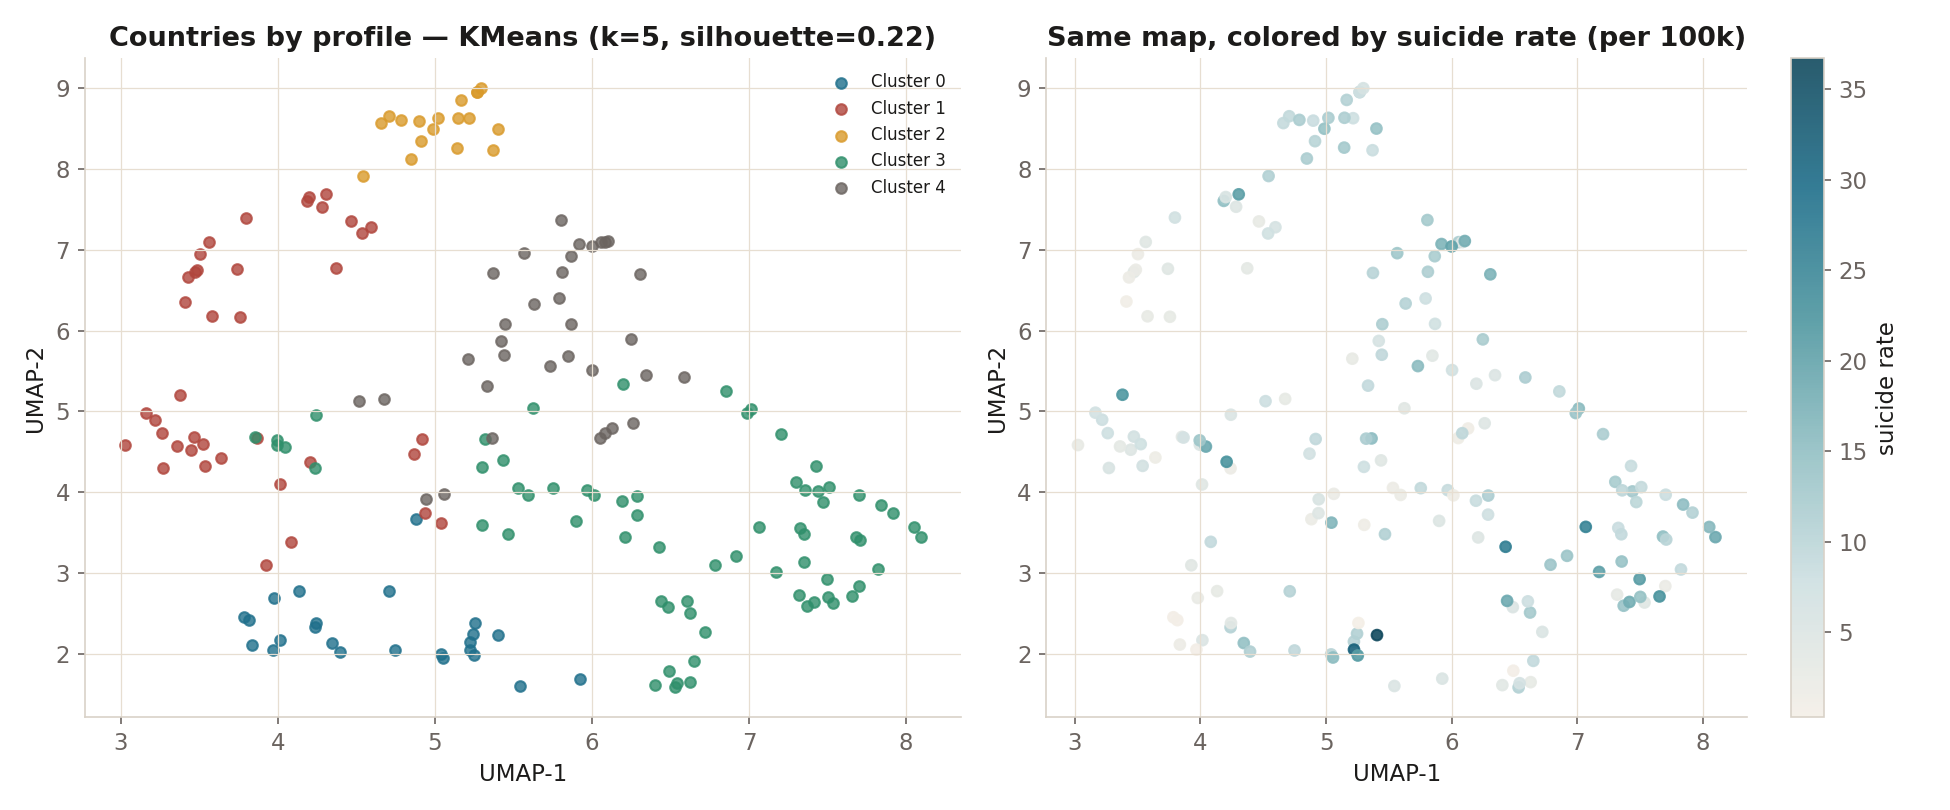
\includegraphics[width=0.86\textwidth]{figures/fig_v1_umap_countries.png}
    \caption{UMAP des pays selon leur profil d'indicateurs de santé mentale.}
    \label{fig:v1_umap_countries}
\end{figure}
\begin{figure}[ht]
    \centering
    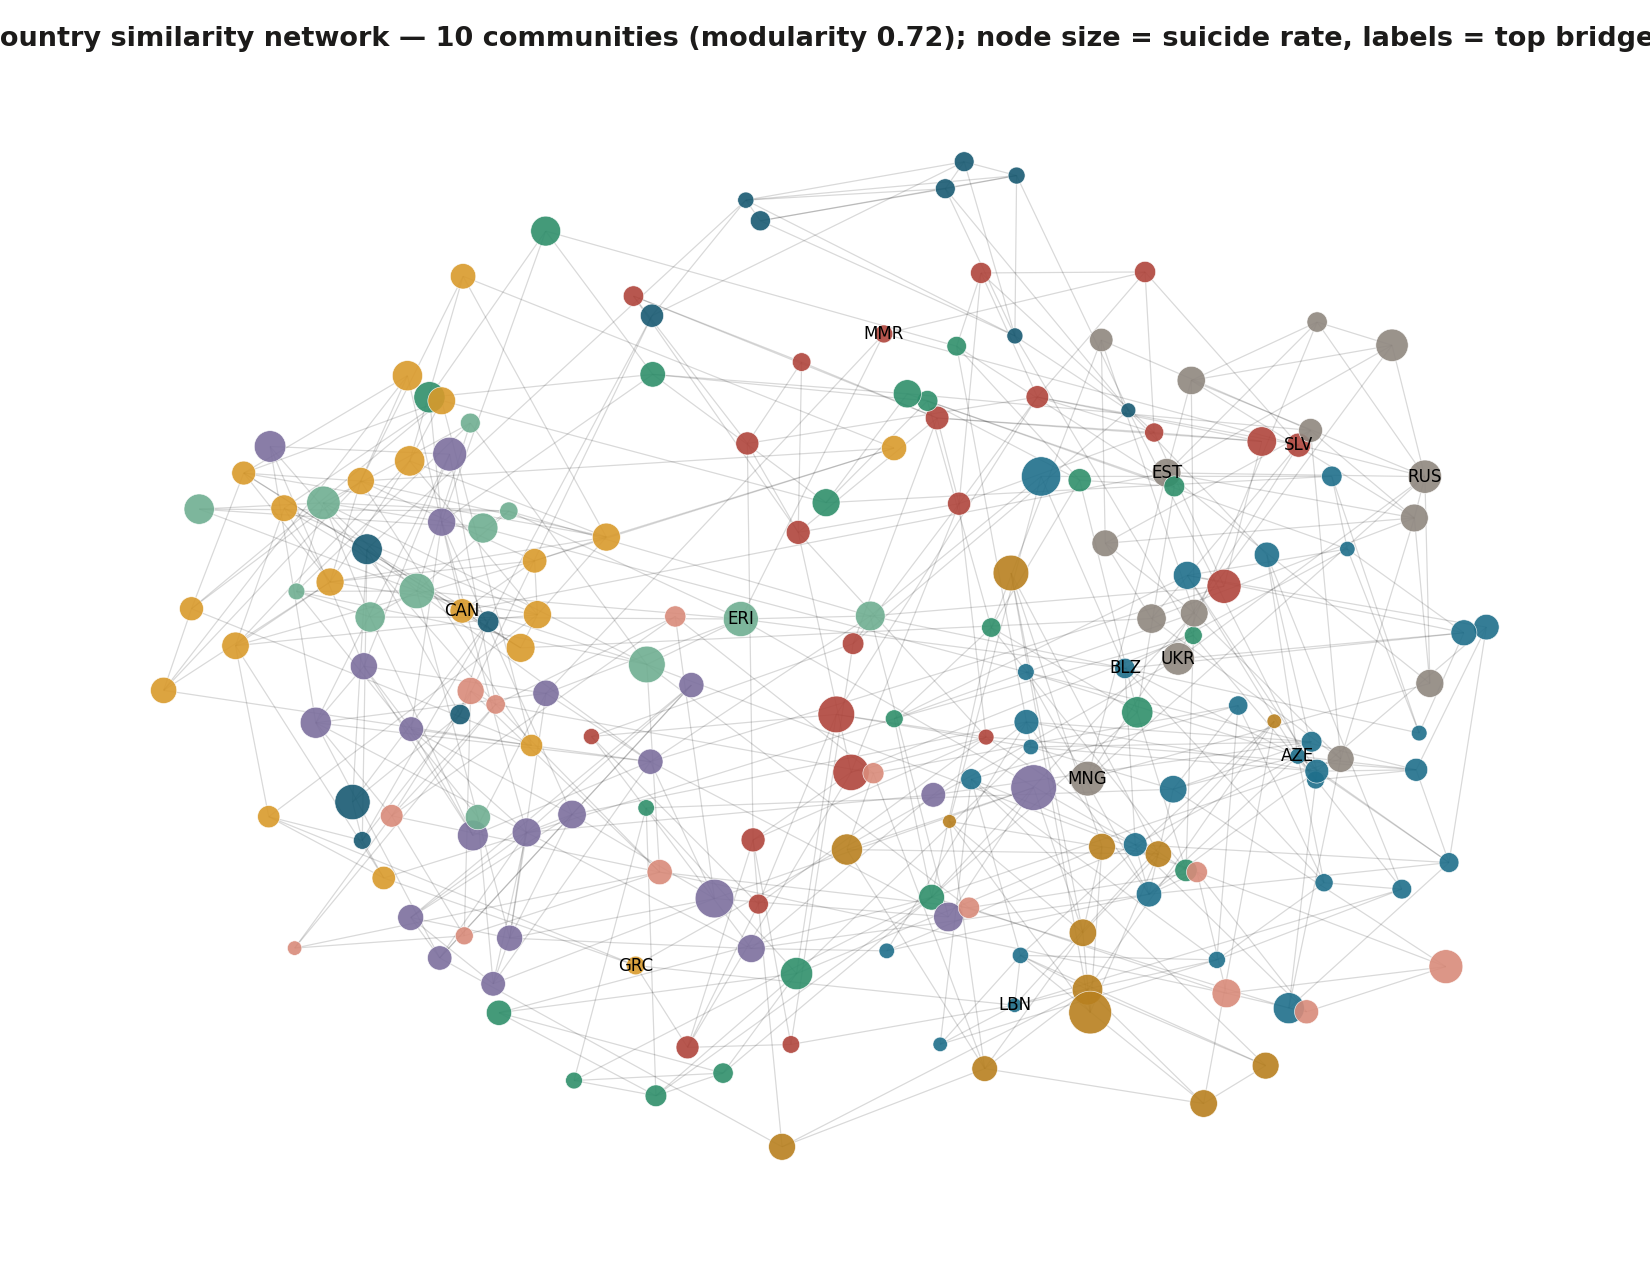
\includegraphics[width=0.86\textwidth]{figures/fig_v1_country_network.png}
    \caption{Réseau de similarité des pays et communautés détectées.}
    \label{fig:v1_country_network}
\end{figure}

\section{Fouille de motifs}
La découverte de sous-groupes (\emph{subgroup discovery}) et des règles
d'association (FP-Growth, après discrétisation en catégories) mettent en évidence
des combinaisons de facteurs associées à un risque élevé, sur données réelles.

\section{Autocorrélation spatiale (réseau)}
Une analyse d'autocorrélation calcule le \textbf{Moran's I} global et les indices
locaux (\textbf{LISA}) sur le graphe de similarité. Le voisinage est défini en
espace de \emph{features} (profils similaires), et non géographiquement --- ce qui
est indiqué explicitement. Le taux brut de suicide est fortement autocorrélé
($I \approx 0{,}21$, $p = 0{,}001$), mais les \textbf{résidus du modèle} ne le sont
pas ($I \approx 0{,}00$, $p = 0{,}42$) : preuve que le modèle sans fuite capture
déjà cette structure.
\begin{figure}[ht]
    \centering
    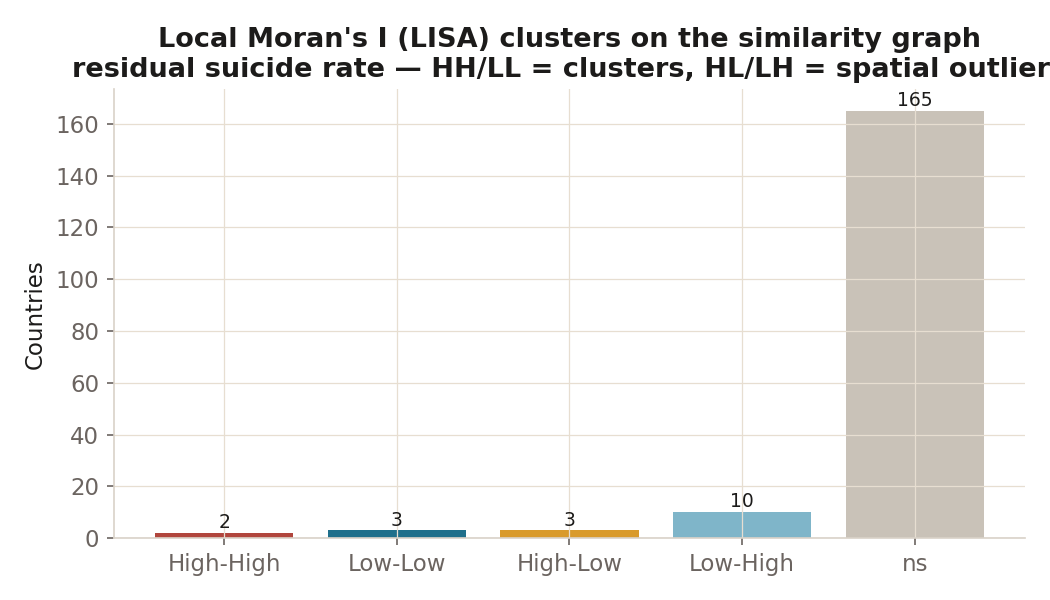
\includegraphics[width=0.9\textwidth]{figures/fig_v1_spatial_lisa.png}
    \caption{Clusters locaux (LISA) des résidus sur le graphe de similarité.}
    \label{fig:v1_spatial_lisa}
\end{figure}
